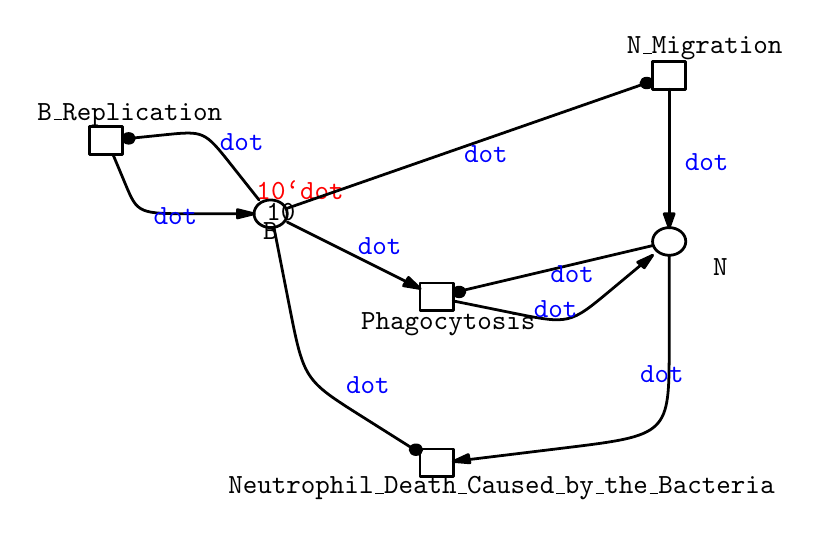
\begin{tikzpicture}[x=0.6pt,y=-0.5pt]

\definecolor{BLACK}{RGB}{0,0,0}
\definecolor{WHITE}{RGB}{255,255,255}
\draw[BLACK, solid, line join=round, line cap=round, line width=1, fill=WHITE]
	(180,140) ellipse[x radius=10, y radius=10];
\draw[BLACK]
	(170,152.5) node[rotate=0, font=\ttfamily\normalsize, BLACK, right=-.25]
	{B};
\draw[BLACK]
	(172,138.5) node[rotate=0, font=\ttfamily\normalsize, BLACK, right=-.25]
	{10};
\definecolor{RED}{RGB}{255,0,0}
\draw[BLACK]
	(166,123.5) node[rotate=0, font=\ttfamily\normalsize, RED, right=-.25]
	{10`dot};
\draw[BLACK, solid, line join=round, line cap=round, line width=1, fill=WHITE]
	(420,160) ellipse[x radius=10, y radius=10];
\draw[BLACK]
	(441,178.5) node[rotate=0, font=\ttfamily\normalsize, BLACK, right=-.25]
	{N};
\draw[BLACK, solid, line join=round, line cap=round, line width=1, fill=WHITE]
	(71,77) rectangle +(20,20);
\draw[BLACK]
	(34,68.5) node[rotate=0, font=\ttfamily\normalsize, BLACK, right=-.25]
	{B\_Replication};
\draw[BLACK, solid, line join=round, line cap=round, line width=1, fill=WHITE]
	(270,190) rectangle +(20,20);
\draw[BLACK]
	(229,219.5) node[rotate=0, font=\ttfamily\normalsize, BLACK, right=-.25]
	{Phagocytosis};
\draw[BLACK, solid, line join=round, line cap=round, line width=1, fill=WHITE]
	(270,310) rectangle +(20,20);
\draw[BLACK]
	(149,338.5) node[rotate=0, font=\ttfamily\normalsize, BLACK, right=-.25]
	{Neutrophil\_Death\_Caused\_by\_the\_Bacteria};
\draw[BLACK, solid, line join=round, line cap=round, line width=1]
	(85,97) -- (92.5,118.5) .. controls (100,140) .. (135,140) -- (170,140);
\draw[BLACK, solid, line join=round, line cap=round, line width=1, fill=BLACK]
	(170,140) -- (160,143) -- (160,137) -- (170,140) -- cycle;
\definecolor{BLUE}{RGB}{0,0,255}
\draw[BLACK]
	(104,141.5) node[rotate=0, font=\ttfamily\normalsize, BLUE, right=-.25]
	{dot};
\draw[BLACK, solid, line join=round, line cap=round, line width=1]
	(190,146) -- (270,194);
\draw[BLACK, solid, line join=round, line cap=round, line width=1, fill=BLACK]
	(270,194) -- (260,192) -- (263,186) -- (270,194) -- cycle;
\draw[BLACK]
	(227,163.5) node[rotate=0, font=\ttfamily\normalsize, BLUE, right=-.25]
	{dot};
\draw[BLACK, solid, line join=round, line cap=round, line width=1]
	(420,170) -- (420,235) .. controls (420,300) .. (355,309.5) -- (290,319);
\draw[BLACK, solid, line join=round, line cap=round, line width=1, fill=BLACK]
	(290,319) -- (299,314) -- (300,320) -- (290,319) -- cycle;
\draw[BLACK]
	(397,255.5) node[rotate=0, font=\ttfamily\normalsize, BLUE, right=-.25]
	{dot};
\draw[BLACK, solid, line join=round, line cap=round, line width=1]
	(290,203) -- (325,211.5) .. controls (360,220) .. (385,195) -- (410,170);
\draw[BLACK, solid, line join=round, line cap=round, line width=1, fill=BLACK]
	(410,170) -- (405,179) -- (401,175) -- (410,170) -- cycle;
\draw[BLACK]
	(333,208.5) node[rotate=0, font=\ttfamily\normalsize, BLUE, right=-.25]
	{dot};
\draw[BLACK, solid, line join=round, line cap=round, line width=1]
	(173,130) -- (156.5,105) .. controls (140,80) .. (115.5,83) -- (91,86);
\draw[BLACK, solid, line join=round, line cap=round, line width=1, fill=BLACK]
	(94.5,85.5) ellipse[x radius=3.5, y radius=3.5];
\draw[BLACK]
	(144,88.5) node[rotate=0, font=\ttfamily\normalsize, BLUE, right=-.25]
	{dot};
\draw[BLACK, solid, line join=round, line cap=round, line width=1]
	(410,163) -- (290,197);
\draw[BLACK, solid, line join=round, line cap=round, line width=1, fill=BLACK]
	(293.5,196.5) ellipse[x radius=3.5, y radius=3.5];
\draw[BLACK]
	(343,183.5) node[rotate=0, font=\ttfamily\normalsize, BLUE, right=-.25]
	{dot};
\draw[BLACK, solid, line join=round, line cap=round, line width=1]
	(182,150) -- (191,205) .. controls (200,260) .. (235,286.5) -- (270,313);
\draw[BLACK, solid, line join=round, line cap=round, line width=1, fill=BLACK]
	(267.5,310.5) ellipse[x radius=3.5, y radius=3.5];
\draw[BLACK]
	(220,263.5) node[rotate=0, font=\ttfamily\normalsize, BLUE, right=-.25]
	{dot};
\draw[BLACK, solid, line join=round, line cap=round, line width=1, fill=WHITE]
	(410,30) rectangle +(20,20);
\draw[BLACK]
	(389,20.5) node[rotate=0, font=\ttfamily\normalsize, BLACK, right=-.25]
	{N\_Migration};
\draw[BLACK, solid, line join=round, line cap=round, line width=1]
	(420,50) -- (420,150);
\draw[BLACK, solid, line join=round, line cap=round, line width=1, fill=BLACK]
	(420,150) -- (417,140) -- (423,140) -- (420,150) -- cycle;
\draw[BLACK]
	(424,102.5) node[rotate=0, font=\ttfamily\normalsize, BLUE, right=-.25]
	{dot};
\draw[BLACK, solid, line join=round, line cap=round, line width=1]
	(190,136) -- (410,44);
\draw[BLACK, solid, line join=round, line cap=round, line width=1, fill=BLACK]
	(406.5,45.5) ellipse[x radius=3.5, y radius=3.5];
\draw[BLACK]
	(291,96.5) node[rotate=0, font=\ttfamily\normalsize, BLUE, right=-.25]
	{dot};
\end{tikzpicture}

